% !TEX root = thesis.tex
\documentclass[12pt,a4paper,titlepage,listof=totoc,bibliography=totoc,chapteratlists=0pt]{scrreprt}
\begin{filecontents*}{\jobname.xmpdata}
	\Keywords{CHANGEME, VR, IOT, TODO}
	\Title{Datenbank Verwaltungstool - Für die Firma Doka}
	\Author{David Altenhofer}
\end{filecontents*}

\setcounter{tocdepth}{2}

\usepackage[utf8]{inputenc}
\usepackage[T1]{fontenc}
\usepackage{amsmath}
\usepackage{amsfonts}
\usepackage{amssymb}
\usepackage[table]{xcolor}
\usepackage{graphicx}
\usepackage[left=3.50cm, right=2.00cm, top=2.00cm, bottom=2.00cm,foot=1cm]{geometry}
\usepackage[splitrule,hang,flushmargin,multiple,bottom]{footmisc}
\usepackage{lmodern, textcomp}
\usepackage{lmodern}
\usepackage{pdfpages}
\usepackage[ngerman]{babel}
\usepackage{multicol}
\usepackage{float}
\usepackage{array,tabularx,booktabs}
\usepackage{ragged2e}
\usepackage{lipsum}
\usepackage{wrapfig}

\usepackage{enumitem}
\newlist{compactitem}{itemize}{3}
\setlist[compactitem,1]{label=\textbullet, nosep,leftmargin=1.5em,labelwidth=*,align=left}
\setlist[compactitem,2]{label=--, nosep,leftmargin=1.5em,labelwidth=*,align=left}
\setlist[compactitem,3]{label=\textopenbullet, nosep,leftmargin=1.5em,labelwidth=*,align=left}
\newlist{compactenum}{enumerate}{3}
\setlist[compactenum,1]{label=\arabic*., nosep,leftmargin=1.5em,labelwidth=*,align=left}
\setlist[compactenum,2]{label=\alph*., nosep,leftmargin=1.5em,labelwidth=*,align=left}
\setlist[compactenum,3]{label=\roman*., nosep,leftmargin=1.5em,labelwidth=*,align=left}
\newlist{compactdesc}{description}{3}
\setlist[compactdesc]{leftmargin=1.5em,labelwidth=*,align=left}

\usepackage{microtype}

\usepackage[parfill]{parskip}

\definecolor{bluekeywords}{rgb}{0.13,0.13,1}
\definecolor{greencomments}{rgb}{0,0.5,0}
\definecolor{redstrings}{rgb}{0.9,0,0}
\definecolor{lightgray}{gray}{0.9}
\definecolor{lightblue}{rgb}{0.93,0.95,1.0}

\usepackage{listings}

\makeatletter
\lstdefinestyle{lststyle}{
	basicstyle=%
	\ttfamily
	\lst@ifdisplaystyle\scriptsize\fi
}
\makeatother

\renewcommand{\lstlistlistingname}{List of Listings}
% TODO: define other languages as needed
\lstset{language=Python,
numbers=left,               
numberstyle=\tiny,          
showspaces=false,
showtabs=false,
breaklines=true,
lineskip=-1pt,
tabsize=2,
showstringspaces=false,
breakatwhitespace=true,
escapeinside={(*@}{@*)},
commentstyle=\color{greencomments},
keywordstyle=\color{bluekeywords}\bfseries,
stringstyle=\color{redstrings},
style=lststyle,
xleftmargin=17pt,
         framexleftmargin=17pt,
         framexrightmargin=5pt,
         framexbottommargin=4pt
}
\lstset{
morekeywords={base,var,in,out,dynamic,from,where,select,orderby,function,\$,group,by,into,yield,async,await,@,None,self,as,elif,with}
}
\lstdefinelanguage{TypeScript}{
	keywords={typeof, new, true, false, catch, function, return, null, switch, var, if, in, while, do, else, case, break, void, number, string, boolean, module, \$, export, for, this},
	keywordstyle=\color{blue}\bfseries,
	ndkeywords={class, export, boolean, throw, implements, import, this},
	ndkeywordstyle=\color{darkgray}\bfseries,
	identifierstyle=\color{black},
	sensitive=false,
	comment=[l]{//},
	morecomment=[s]{/*}{*/},
	commentstyle=\color{purple}\ttfamily,
	stringstyle=\color{red}\ttfamily,
	morestring=[b]',
	morestring=[b]"
}
\usepackage{caption}
\DeclareCaptionFont{white}{\color{white}}
\DeclareCaptionFormat{listing}{\colorbox[cmyk]{0.43, 0.35, 0.35,0.01}{\parbox{\textwidth}{\hspace{10pt}#1#2#3}}}
\captionsetup[lstlisting]{format=listing,labelfont=white,textfont=white} 
\captionsetup[table]{justification=centering, singlelinecheck=false}

\usepackage{subcaption}

\usepackage{setspace}
\newcommand{\MSonehalfspacing}{%
	\setstretch{1.44}%  default
	\ifcase \@ptsize \relax % 10pt
	\setstretch {1.448}%
	\or % 11pt
	\setstretch {1.399}%
	\or % 12pt
	\setstretch {1.433}%
	\fi
}

\newcommand{\setauthor}[1]{\ohead[]{#1}}

\usepackage[automark]{scrlayer-scrpage}
\pagestyle{scrheadings}
\automark{chapter}
\renewcommand\sectionmark[1]{\markright{\MakeMarkcase {\thesection\hskip .5em\relax#1}}}
\rohead{\ifnum\expandafter\pdfstrcmp\botmark=0 \rightmark\else\leftmark{} --- \rightmark\fi}
\ihead[]{\headmark}
\chead[]{}
\ohead{}
\cfoot[]{}
\ofoot[\pagemark]{\pagemark}
\setheadsepline{.1pt}

\usepackage[hyphens]{url}

\usepackage[a-1b]{pdfx}

\usepackage{hyperref}
\hypersetup{pdfa}

\usepackage[nonumberlist,toc,nopostdot]{glossaries}

\usepackage{chngcntr}
\counterwithout{footnote}{chapter}
\counterwithout{figure}{chapter}
\counterwithout{table}{chapter}
\AtBeginDocument{
	\counterwithout{lstlisting}{chapter}
	\urlstyle{sf}
}
\newcounter{RPages}

\makeatletter
\def\bstctlcite{\@ifnextchar[{\@bstctlcite}{\@bstctlcite[@auxout]}}
\def\@bstctlcite[#1]#2{\@bsphack
	\@for\@citeb:=#2\do{%
		\edef\@citeb{\expandafter\@firstofone\@citeb}%
		\if@filesw\immediate\write\csname #1\endcsname{\string\citation{\@citeb}}\fi}%
	\@esphack}
\makeatother

\clubpenalty=10000 
\widowpenalty=10000
\displaywidowpenalty=10000
\interfootnotelinepenalty=10000

\title{Datenbank Verwaltungstool - Für die Firma Doka}
\author{David Altenhofer}

\makeindex
\makeglossaries
\begin{document}
\bstctlcite{IEEEexample:BSTcontrol}
\newcommand{\reminder}[1]
{ \textcolor{red}{<[{\bf\marginpar{\mbox{$<==$}} #1 }]>} }
\newcommand{\icode}[1]{\lstinline$#1$}
%\urlstyle{same}
%\setstretch{1.5}
\setstretch {1.433}
\renewcommand{\arraystretch}{1.2}

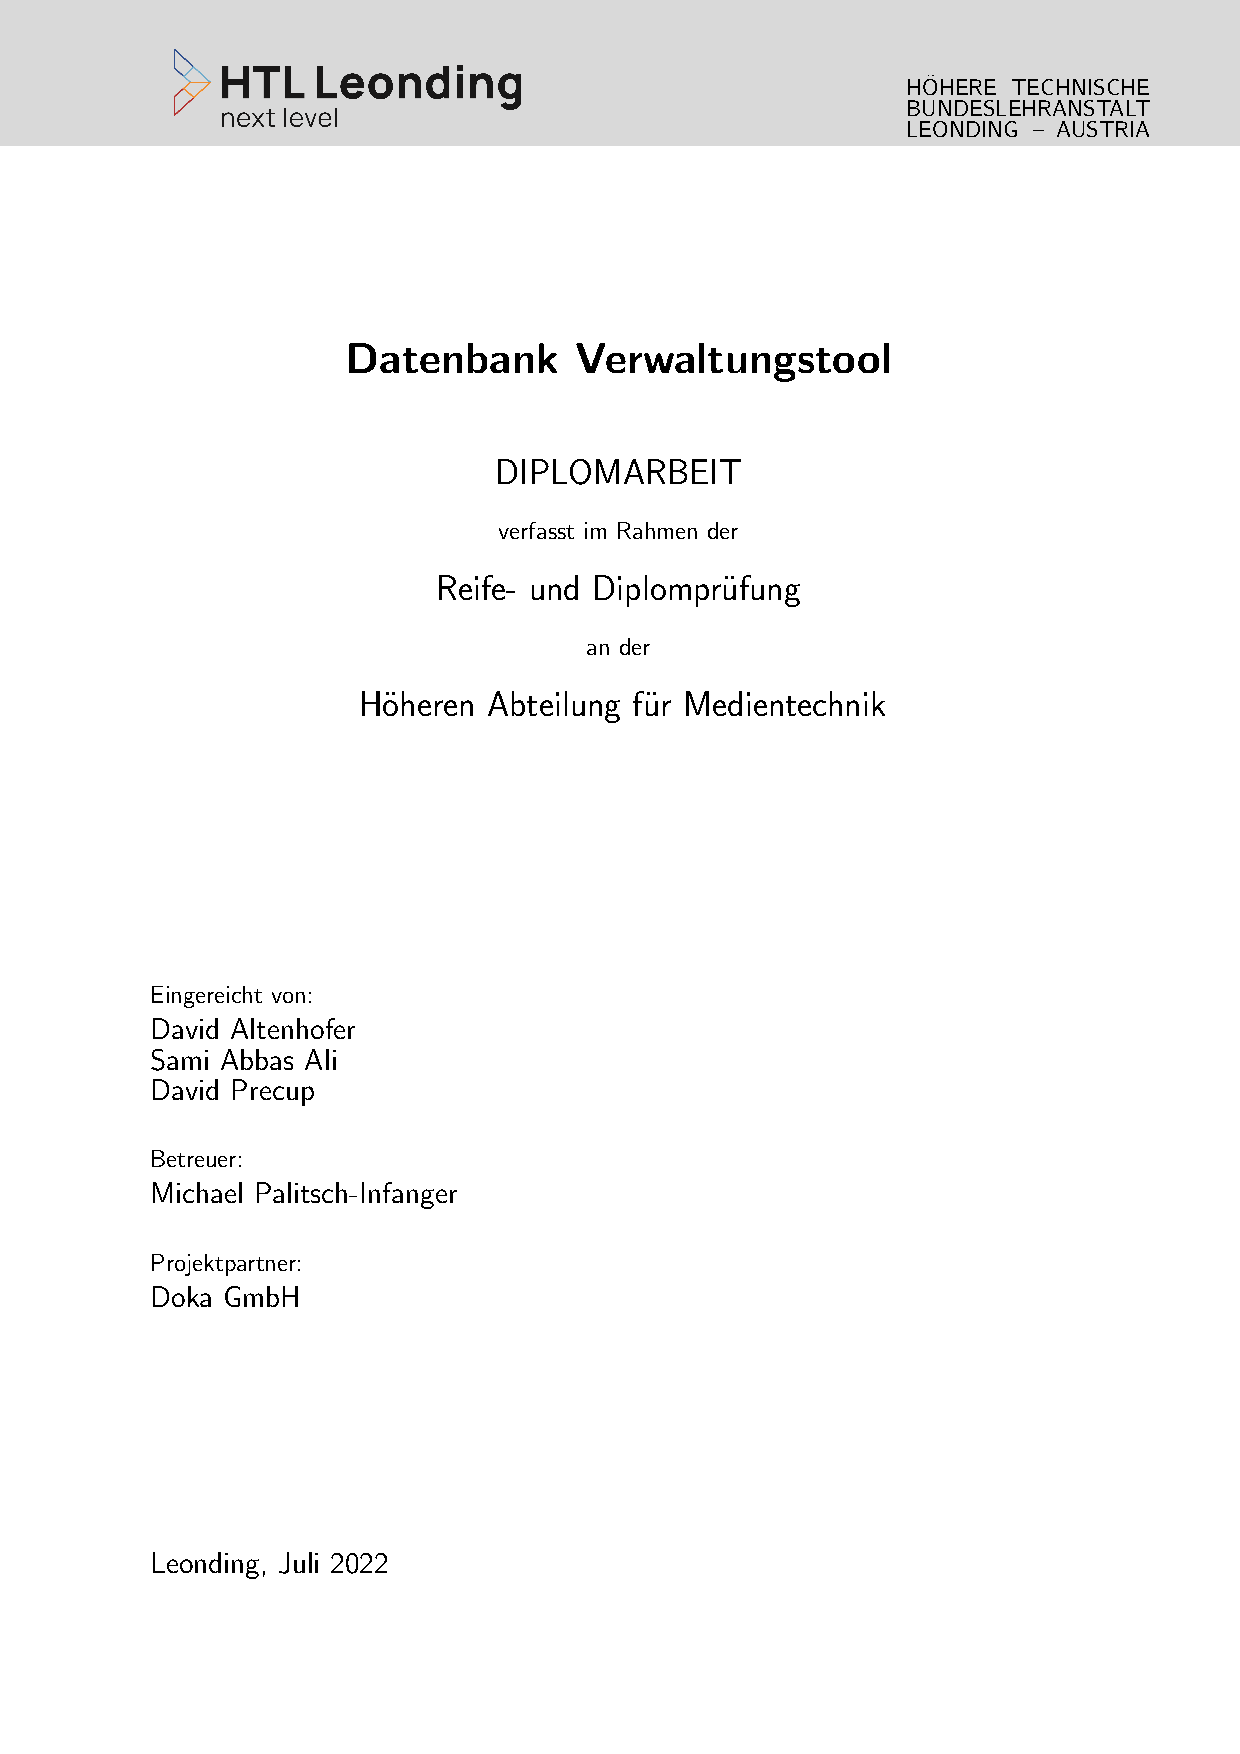
\includepdf{./titlepage/coversheet}
\pagenumbering{Roman}
\newpage
\thispagestyle{empty}
\vspace{3cm}
~ \\ \\
Ich erkläre an Eides statt, dass ich die vorliegende Diplomarbeit selbstständig und ohne fremde Hilfe verfasst, andere als die angegebenen Quellen und Hilfsmittel nicht benutzt bzw. die wörtlich oder sinngemäß entnommenen Stellen als solche kenntlich gemacht habe.

Die Arbeit wurde bisher in gleicher oder ähnlicher Weise keiner anderen Prüfungsbehörde vorgelegt und auch noch nicht veröffentlicht.

Die vorliegende Diplomarbeit ist mit dem elektronisch übermittelten Textdokument identisch.
\vspace{3cm}
% Hier kommt die Unterschrift drüber
\begin{tabbing}
Leonding, April 2022 \hspace{5cm} S. Schwammal \& S. Schwammal
\end{tabbing}
\vspace{10cm}
\newpage
\setcounter{page}{1}

\begin{spacing}{.5}
  \chapter*{Abstract}
\end{spacing}
The Doka company offers software packages to their customers. Here is the administration
still very much in need of improvement. The process of adding new software packages,
works as follows: creating new packages, editing and deleting
takes place directly via the database, which means that there is no administration program
to date. Since everything runs through the database, it becomes clean
work prevented. That's why we were commissioned by the Doka company to create a
Database Management System based on the JavaScript library React. 
Before some terms need to be explained:
\\
\\
It should be possible to manage the following tables that have these properties: 
\\
\\
- InstallablePackage is the main table, consists of several Installables and
can have a description (InstallablaPackagesDesciptions) in multiple languages. 
\\
- An Installable has an InstallableSyncTemplate and can have an InstallableExecutablePaths.
\\
\\
The program should have the following functions:
\\
\\
- Viewing, installing, adding, editing and deleting so-called
\\
Installables / InstallablePackages / InstallableSyncTemplates / InstallableExecutablePaths 
- Exporting the current configuration 
\\
- Importing a JSON file,
where to see the difference of the imported file and the current configuration 
\\
- Reset the cache in the backend

\begin{figure}
  \centering
  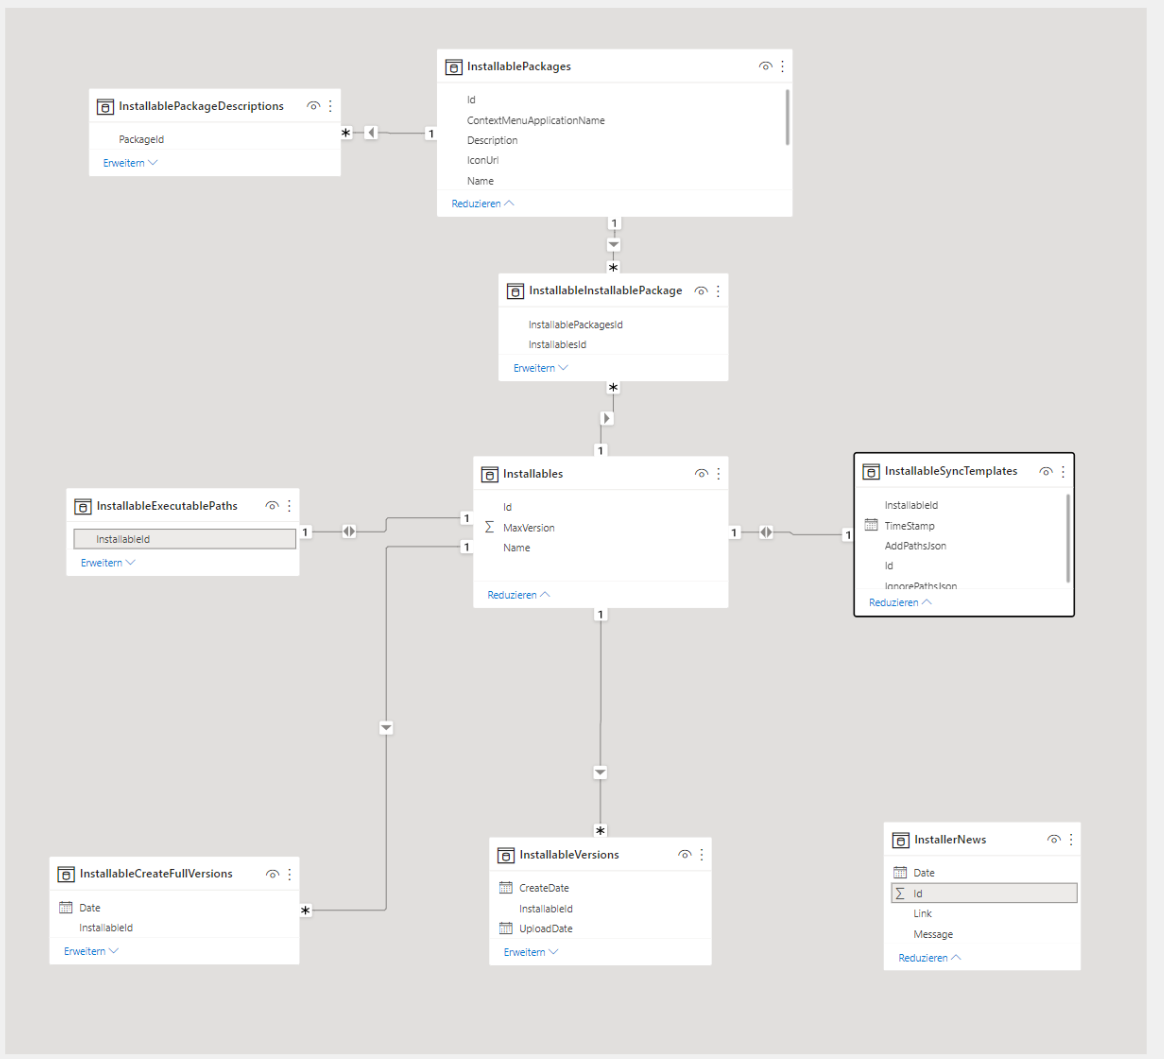
\includegraphics[width=.94\textwidth]{pics/erd.png}
  \caption{\label{fig:The-caption} ERD}
\end{figure}

\newpage
\begin{spacing}{.5}
  \chapter*{Zusammenfassung}
\end{spacing}
Die Firma Doka bietet Softwarepakete an deren Kunden an. Dabei ist das Verwalten noch sehr verbesserungswürdig.
Der Prozess des hinzufügens von neuen Softwarepaketen, läuft wiefolgt ab:
Das Erstellen von neuen Paketen, das Editieren sowie das Löschen erfolgt direkt über die Datenbank, das bedeutet, dass
es kein Verwaltungsprogramm bis dato gibt. Dadruch, dass alles über die Datenbank abläuft, wird das saubere Arbeiten
verhindert. Deshalb wurden wir von der Firma Doka dazu beauftragt, ein Verwaltungssystem basierend auf der JavaScript library
React zu programmieren. Davor müssen einige Begriffe noch erklärt werden:
\\
\\
Folgende Tabellen sollen verwaltet werden können, die diese Eigenschaften haben:
\\
\\
- InstallablePackage ist die wichtigste Tabelle, besteht aus mehreren Installables und kann Beschreibung (InstallablaPackagesDesciptions) auf mehreren Sprachen haben.
\\
- Ein Installable hat ein InstallableSyncTemplate und kann ein InstallableExecutablePaths.
\\
\\
Dabei soll das Programm folgende Funktionen haben:
\\
\\
- Das Anzeigen, Installieren, Hinzufügen, Bearbeiten und Löschen von sogenannten Installables / InstallablePackages / InstallableSyncTemplates / InstallableExecutablePaths
\\
- Das Exportieren der aktuellen Konfiguration
\\
- Importieren eines JSON Dateis, wo die Differenz der importierten Datei und der aktuellen Konfiguration zu sehen ist
\\  
- Reseten des Cache im Backend

\begin{figure}
  \centering
  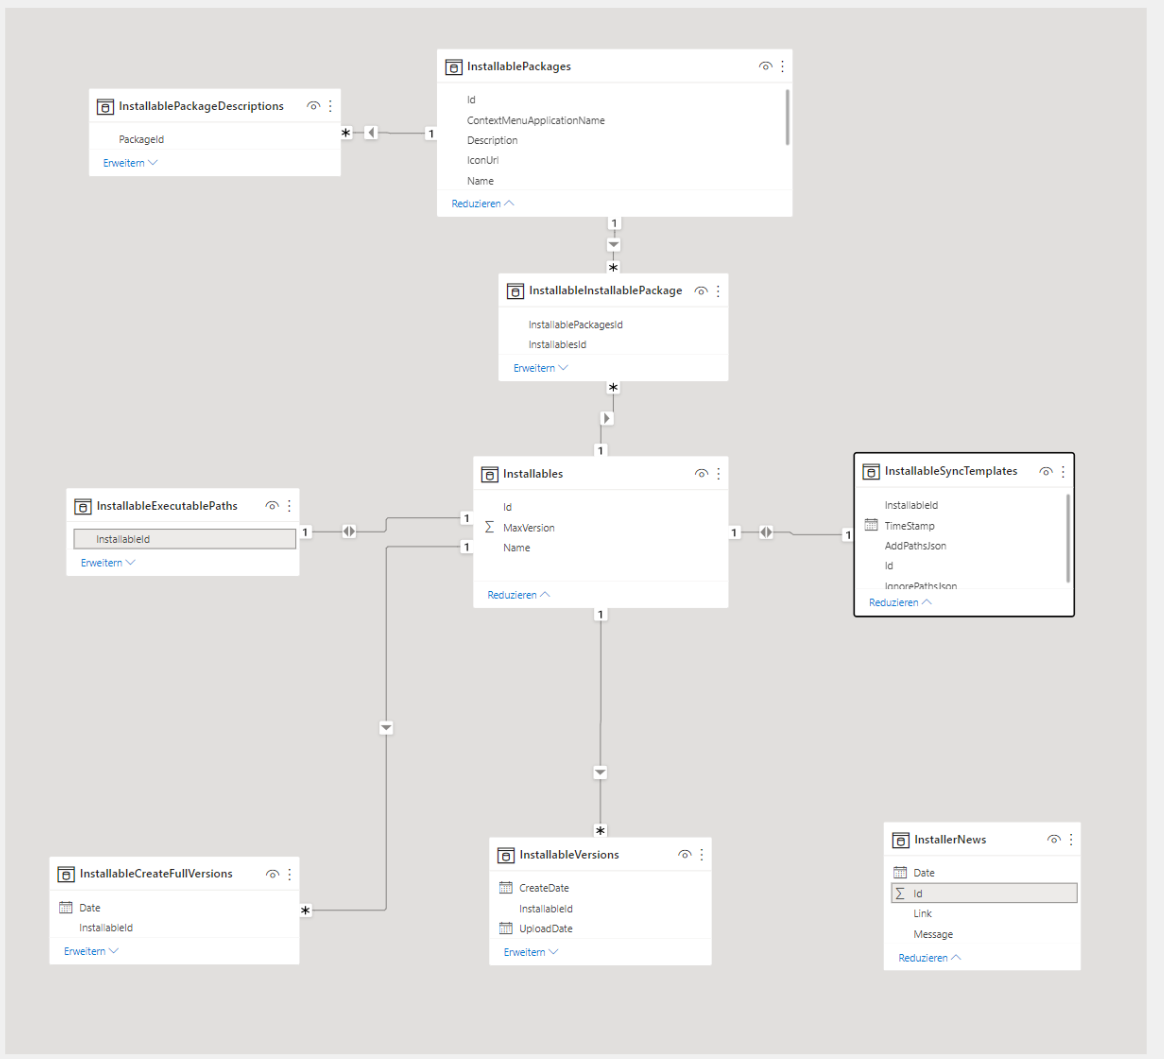
\includegraphics[width=.94\textwidth]{pics/erd.png}
  \caption{\label{fig:The-caption}ERD}
\end{figure}

%\emph{Bitte auf keinen Fall mit der Zusammenfassung verwechseln, die den Abschluss der Arbeit bildet!}
\newpage
\begin{spacing}{1}
    \chapter*{Autoren der Diplomarbeit}
  \end{spacing}
\setauthor{David Altenhofer}

\textbf{David Altenhofer}

\textbf{Aufgabenbereich}
Frontend und Authentifizierungslogik

\begin{flushleft}
Name: David Altenhofer\\
Geburtsdatum: 8. Juli 2003\\
E-Mail: david.altenhofer@gmail.com
\end{flushleft}

\subsection*{Bildungsweg}
2009 bis 2010 Vorschule Karlhof\\
2010 bis 2014 Volkschule Karlhof\\
2014 bis 2018 Europagymnasium Auhof (Kepler-Zweig)\\
Seit September 2018 in der HTL-Leonding (Medientechnik) 

\subsection*{Berufliche Erfahrung:}
Sommer 2023 Doka GmbH, Frontend Entwickler

\subsection*{Sprachliche Kenntnisse:}
Deutsch Muttersprache\\
Englisch

\newpage
\begin{spacing}{.5}
    \chapter*{Danksagung}
  \end{spacing}
An dieser Stelle möchten wir uns bei denen bedanken, die uns bei der Durchfuhrung dieses Projektes 
beraten und unterstützt haben.
Besonderer Dank, gilt Alex und Mathias, die als Mitarbeiter unserer Partnerfirma Doka, uns im Laufe 
des Projekts fachlich geholfen haben, bei der Planung als auch bei der Durchführung und Lösung von Hindernissen.
Ein weiteres Dankeschön an die Firma Doka, die uns unser Diplomarbeitsprojekt im Rahmen eines 
Praktikums im Sommer zur Verfügung gestellt haben.

Zu guter letzt möchten wir uns noch bei unserem Betreuer Herrn Prof Palitsch-Infanger, 
für die Beratung und Begleitung dieser Diplomarbeit, bedanken.



\pagestyle{plain}

\renewcommand{\lstlistlistingname}{Quellcodeverzeichnis}

\tableofcontents
\newpage
\setcounter{RPages}{\value{page}}
\setcounter{page}{0}
\pagenumbering{arabic}
\pagestyle{scrheadings}

\begin{spacing}{1}
\chapter{Einleitung}\label{chapter:introduction}
\end{spacing}


\section{Ausgangssituation}
\label{sec: initial_situation}
\setauthor{David Altenhofer}
Seit Jahren müssen die Mitarbeiter der Firma die Datenbank
Einträge sehr umständlich ändern, da kein User Interface dafür 
vorhanden ist. Unser Ziel war es, genau das zu Ändern. Ich habe gemeinsam
mit meinem Team ein Web-Frontend erstellt, welches das Hinzufügen, Bearbeiten
und Löschen der Einträge in der Datenbank um ein vielfaches vereinfacht.
Nun kann auf das unpraktische Verwenden von Swagger verzichtet werden und auf ein paar 
wenige Klicks reduziert werden. 
\\
\\
Gegeben war bereits ein fertiges Backend mit einer API

\clearpage  

\begin{figure}[p]
    \centering
    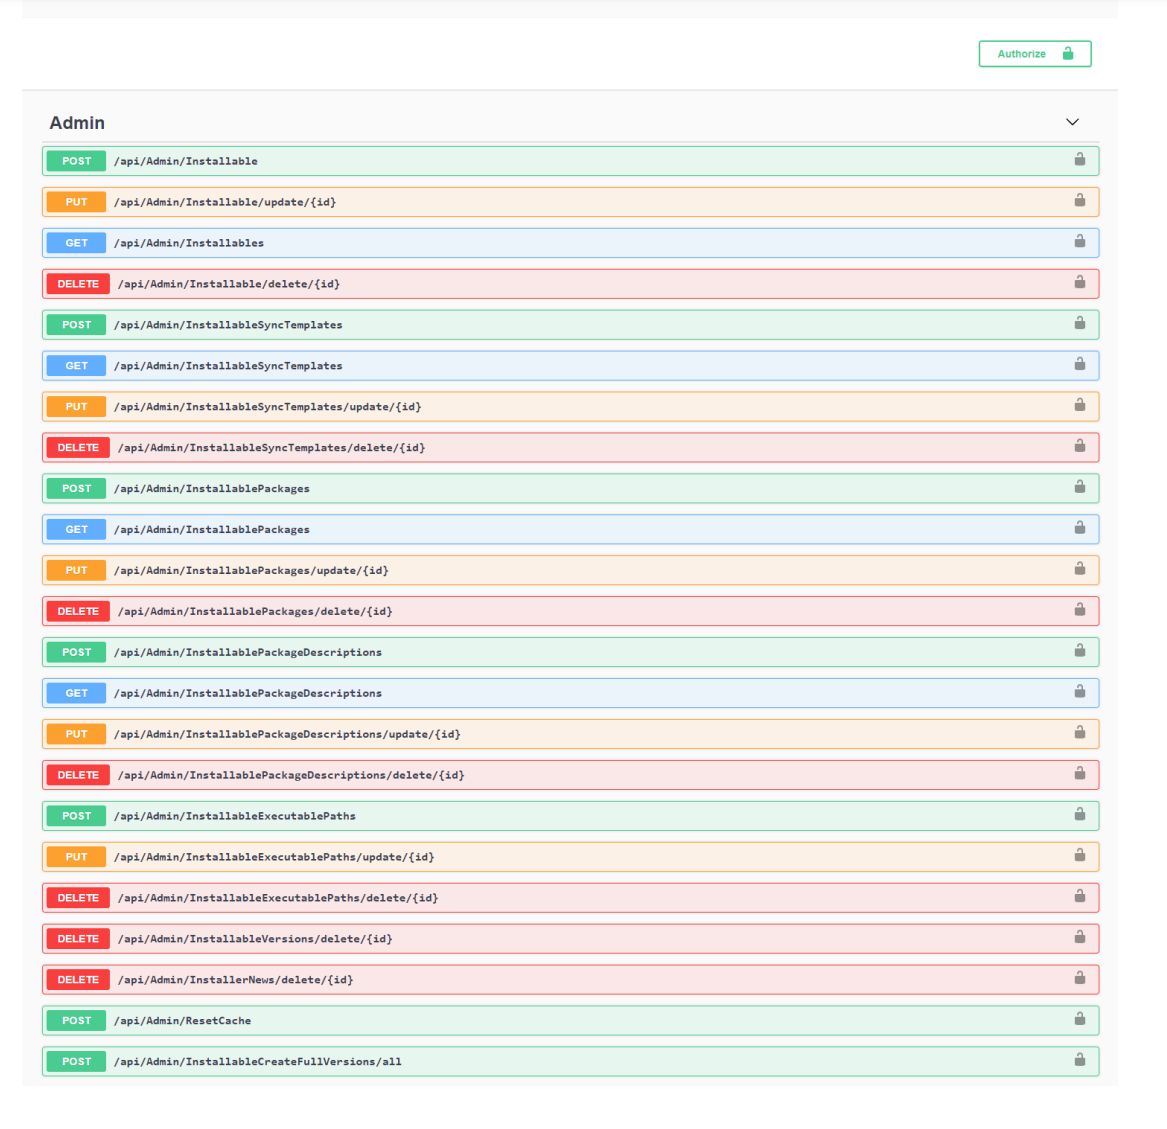
\includegraphics[width=.94\textwidth]{pics/swagger01.PNG}
    \caption{Swagger UI - Endpoints}
\end{figure}
\clearpage
\begin{figure}[p]
    \centering
    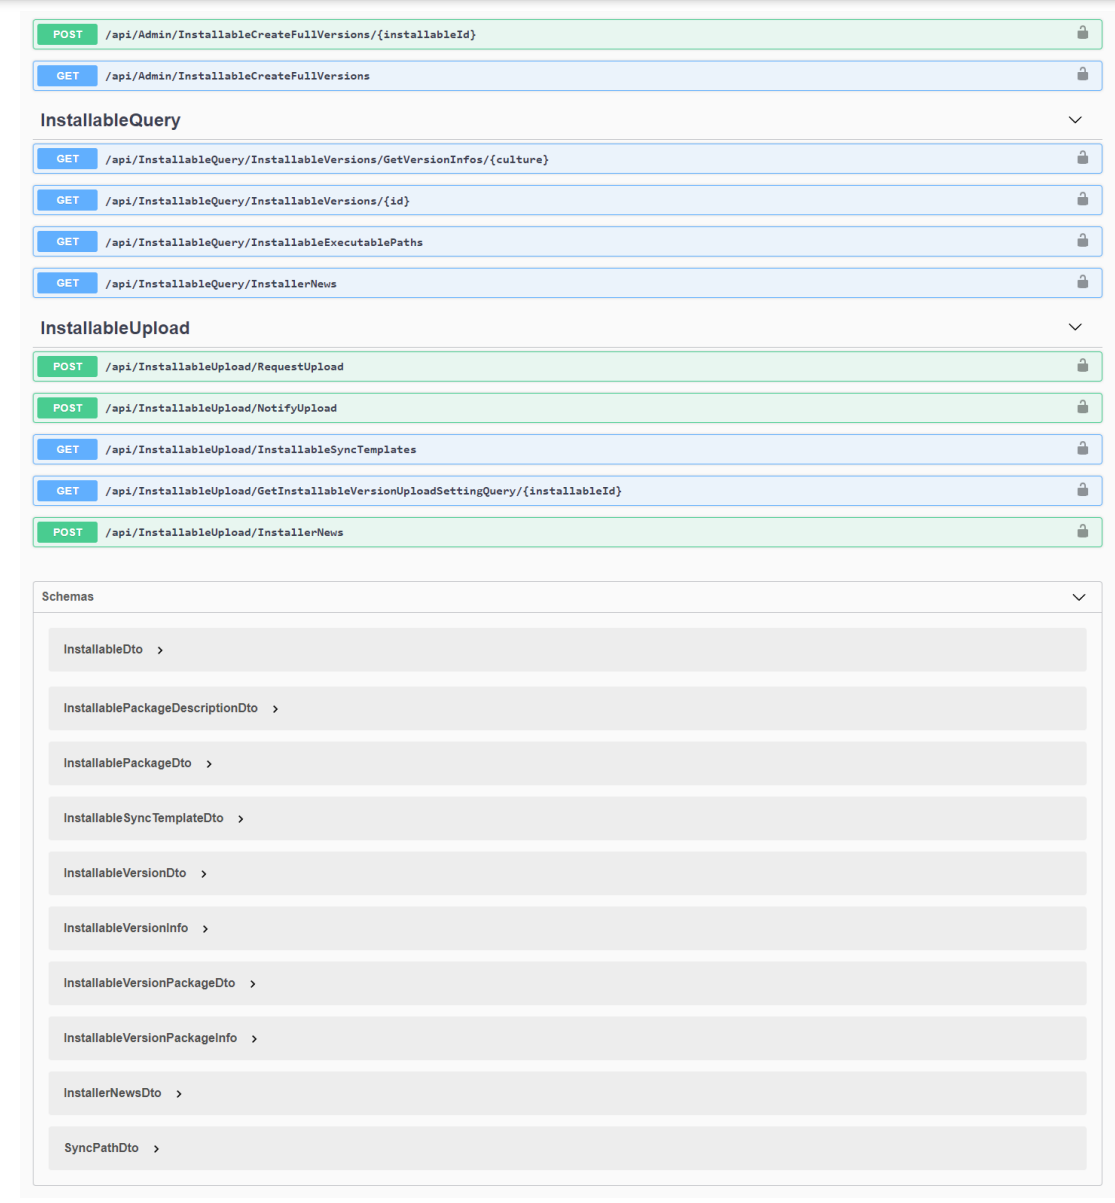
\includegraphics[width=.94\textwidth]{pics/swagger02.PNG}
    \caption{Swagger UI - Endpoints}
\end{figure}

\clearpage

\section{Aufgabenstellung}
\setauthor{David Altenhofer}
Um den Umgang mit der Datenbank für alle Mitarbeiter zu vereinfachen, soll ein leicht verständliches, inuitives Interface entwickelt werden.
Die Web-Anwendung darf nur für autorisierte Benutzer in der Abteilung der Firma verfügbar sein. Deswegen ist eine Authentifizierungslogik zu 
implementieren. Erst nach erfolgreichen Anmelden mit einem gültigen Doka-Account, soll die Website erreichbar sein und Änderungen in der Datenbank
durchgeführt werden können.


\section{Zielsetzung}
\setauthor{David Altenhofer}
Die Web-Anwendung soll in einem ansprechenden Design entwickelt werden und ein
leicht verständlicher unkomplizierter Umgang muss auch für Nicht-Fachleute gegeben
sein. 


	
\begin{spacing}{1}
\chapter{Technologien}\label{chapter:tech}
\end{spacing}

\section{React}
\setauthor{David Altenhofer}
React ist eine \textbf{JavaScript-Programmbibliothek} zur Erstellung von webbasierten Benutzeroberflächen. 
Jede React-Webanwendung besteht aus wiederverwendbaren Komponenten, die Teile der Benutzeroberfläche bilden – wir können 
eine separate Komponente für unsere Navigationsleiste haben, eine für die Fußzeile, eine andere für den Hauptinhalt und so weiter. 

Diese wiederverwendbaren Komponenten machen die Entwicklung einfacher, weil man wiederkehrenden Code nicht wiederholen muss. 
Man muss nur die Logik erstellen und die Komponente in jeden Teil des Codes importieren, in dem sie benötigt wird.
React ist außerdem eine Single-Page-Anwendung. Anstatt also jedes Mal, wenn eine neue Seite gerendert werden soll, eine Anfrage 
an den Server zu senden, wird der Inhalt der Seite direkt von den React-Komponenten geladen. Das führt zu einem schnelleren 
Rendering ohne Neuladen der Seite.

In den meisten Fällen wird für die Erstellung von React-Apps die Syntax JSX (JavaScript XML) verwendet, eine Syntaxerweiterung 
von JavaScript. Damit kann man die Logik von JavaScript und die Logik der Benutzeroberfläche auf einzigartige Weise kombinieren. 
Mit JSX muss kein DOM integriert werden, weil man einfach Methoden wie \textbf{document.getElementById}, \textbf{querySelector} 
und andere DOM-Manipulationsmethoden verwendet.
Die Verwendung von JSX ist zwar nicht obligatorisch, aber sie macht die Entwicklung von React-Anwendungen einfacher.


\begin{figure}[ht!]
    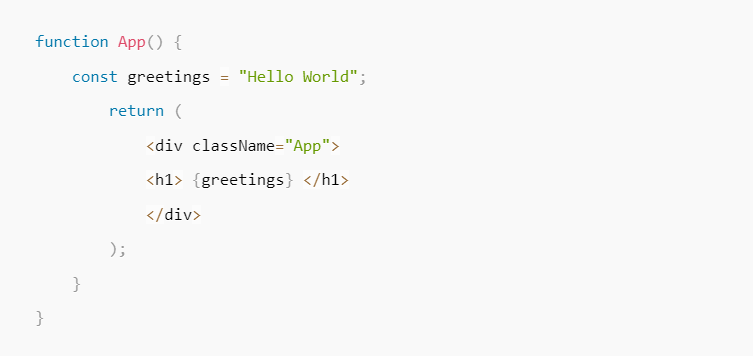
\includegraphics[width=.94\textwidth]{pics/jsx-example.PNG}
    \caption{\label{fig:The-caption}JSX-Example in React \cite{APCW2006}}
  \end{figure}

Im oberen Code-Beispiel wird eine funktionale React-Komponente verwendet, um ein Stück Text im Browser darzustellen. 
Der Name der Komponente ist \textbf{App}. Es wird eine Variable vor der Funktion \textbf{render()} erstellt.
Diese Variable wird mit geschweiften Klammern an das Markup übergeben. Das ist kein HTML, sondern die 
Syntax für das Schreiben von Code mit JSX.

\clearpage

\section{Tailwind CSS}
\setauthor{David Altenhofer}
Tailwind CSS ist ein Utility-First-CSS-Framework. Es stellt vorgefertigte CSS-Klassen bereit, die verwendet 
werden können, um HTML-Elemente schnell und einfach zu gestalten. Im Vergleich mit anderen CSS-Frameworks, 
die vorgefertigte UI-Komponenten bereitstellen, fokussiert sich Tailwind mehr auf Low-Level-Bausteine wie 
Abstände (Paddings und Margins), Schriftarten und Farbe, um benutzerdefinierte Styles zu erstellen.

Entwickler können vorgefertigte CSS-Klassen hinzufügen, anstatt für jedes Element benutzerdefiniertes CSS zu 
schreiben. Das beschleunigt nicht nur den Entwicklungsprozess, sondern kann sich auch positiv auf die Performance 
auswirken. Die Dokumentation von Tailwind CSS ist umfangreich und die große Community erleichtert den Einstieg und 
bietet Unterstützung.

\begin{figure}[ht!]
    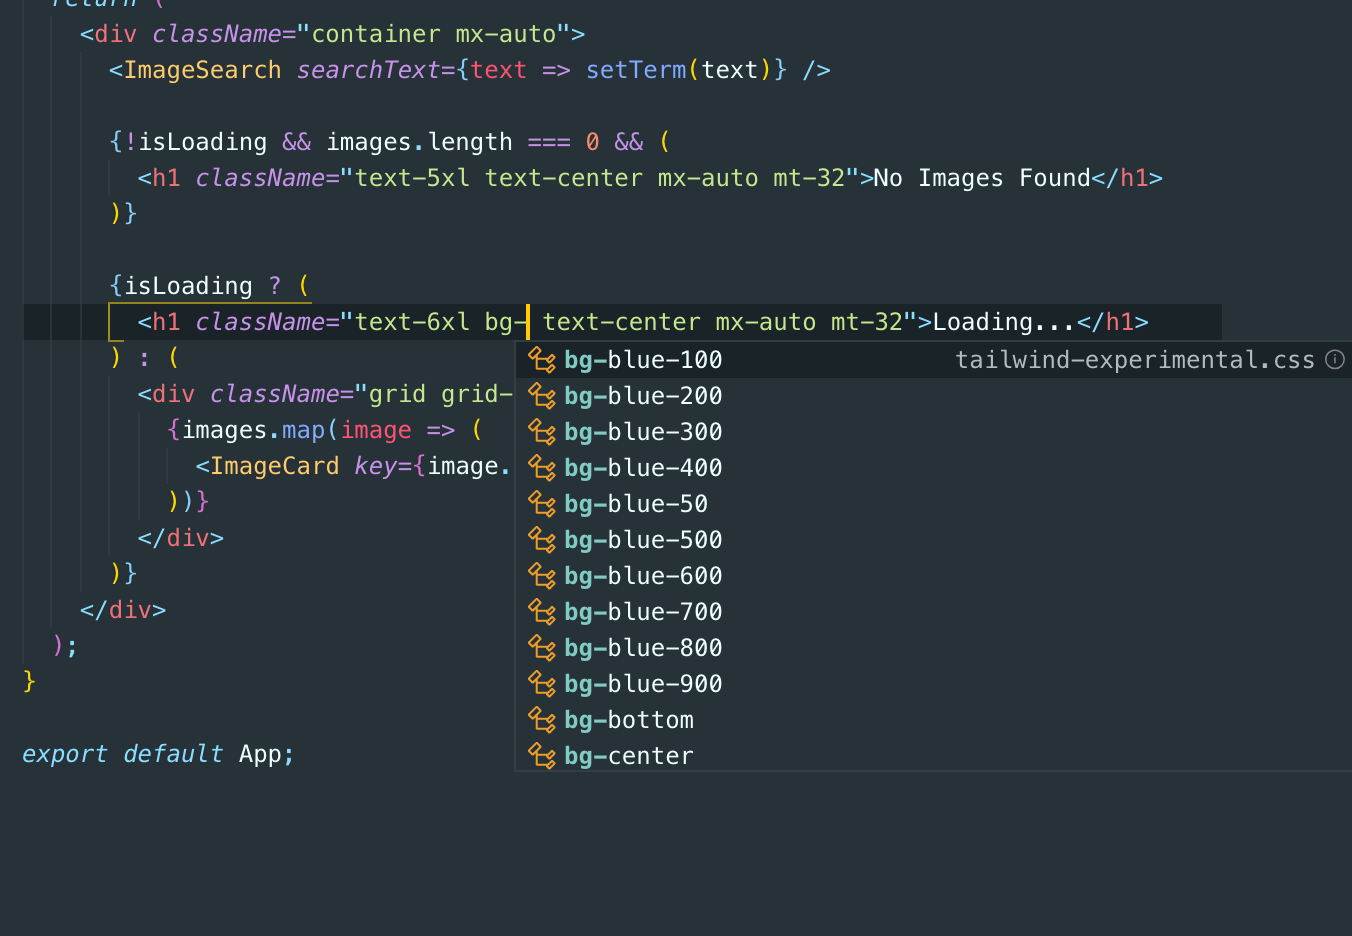
\includegraphics[width=.94\textwidth]{pics/tailwindCSS-class-showcase.png}
    \caption{\label{fig:The-caption}Tailwind - vorgefertigte CSS-Klassen \cite{APCW2006}}
  \end{figure}

\section{Dev Ops}
\setauthor{David Altenhofer}

\section{Adobe XD}
\setauthor{David Altenhofer}


	
\begin{spacing}{1}
\chapter{Umsetzung}\label{chapter:implementation}
\end{spacing}
\section{Planung}
\setauthor{David Altenhofer}
Sobald die Festlegung und die Aufteilung der Arbeitspakete in der Firma geregelt waren, wurde mit dem Use-Case-Diagramm begonnen.
Es haben sich alle Teamkollegen der Diplomarbeit daran beteiligt und nach einigen Änderungen, Diskussionen und Empfehlungen 
war das Use-Case-Diagramm nach zwei Tagen finalisiert.
\\
\subsection*{Was ist ein Use-Case-Diagramm?}
Ein Use-Case-Diagramm ist eine von vielen Arten der Unified Modeling
Language (UML). Es wird verwendet um die funktionalen Anforderungen eines 
Systems beziehungsweise einer Anwendung zu visualisieren. Das Diagramm funktioniert 
so, dass ein Benutzer mit einem System interagiert, indem es Anwendungsfälle 
(Use Cases) und Akteure (Benutzer) zeigt, die den Anwendungsfall durchlaufen.
Solche Diagramme sind besonders nützlich, für das Verständnis der Funktionalität im 
Projekt ohne dabei viel technisches Fachwissen vorauszusetzen.\cite{APCW20018}

\begin{figure}[ht!]
    \centering
    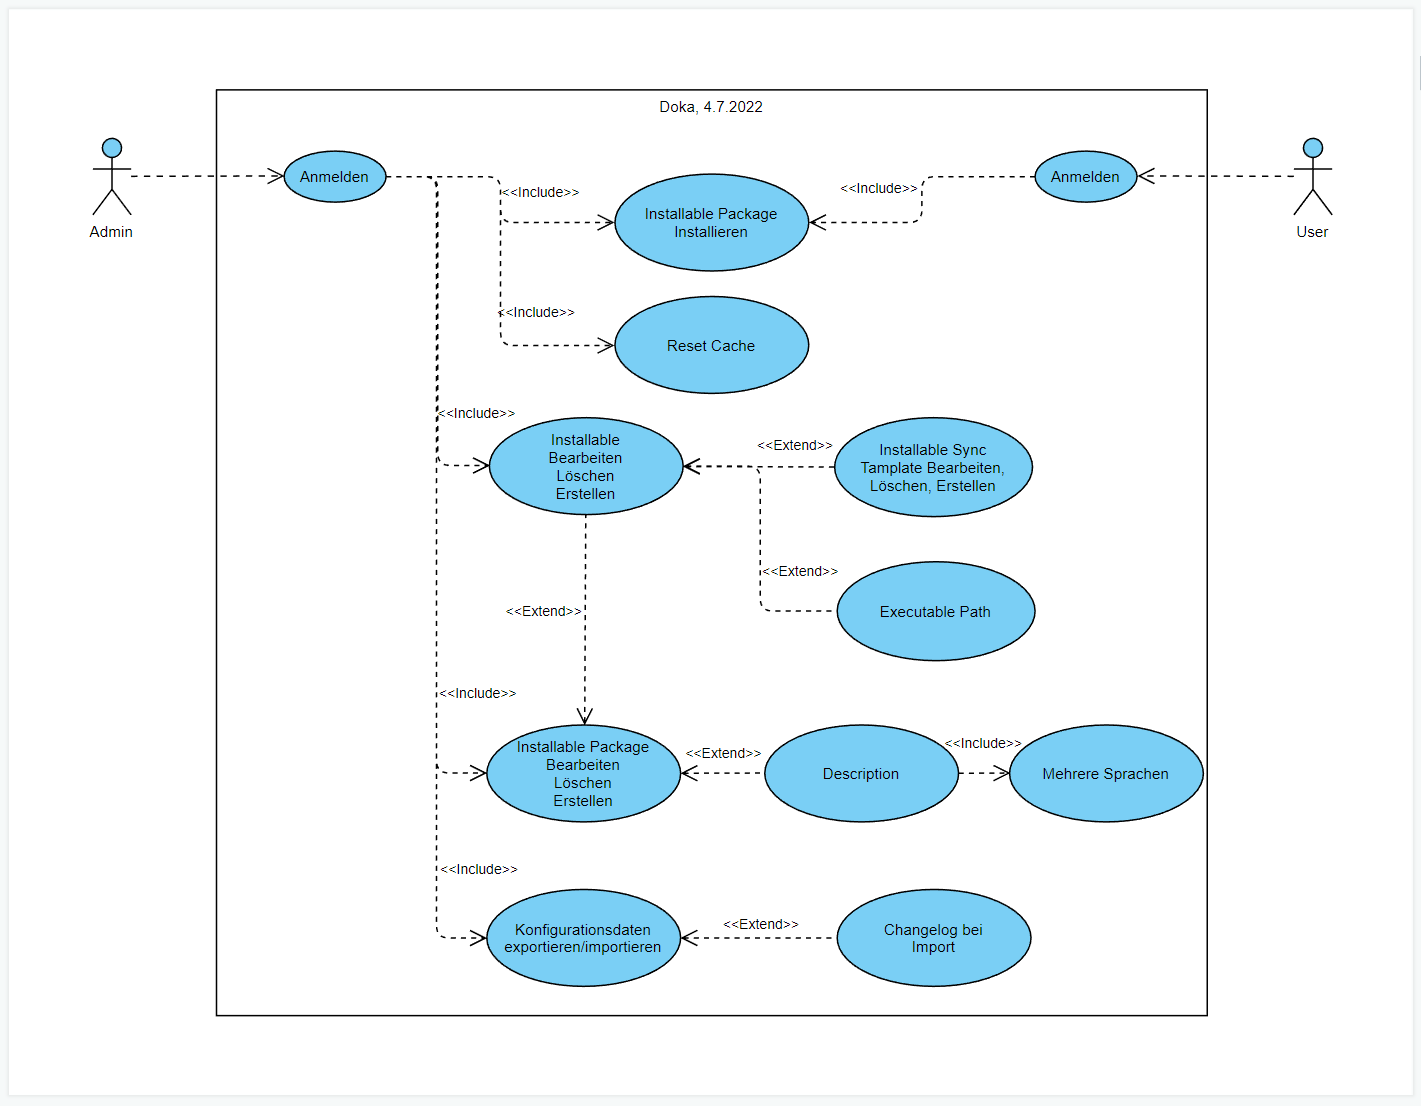
\includegraphics[scale=0.3]{pics/UCD.png}
    \caption{\label{fig:The-caption}Use-Case-Diagramm des Projekts}
    \label{fig:impl:use-case-diagramm}
  \end{figure}
\newpage

\subsection{Scrum}
Für den Entwicklungsprozess wurde Scrum als agiles Vorgehensmodell im Projekt angewandt.
Scrum ist eine Methode für agiles Projektmanagement. Es wird 
oft von Softwareentwickler-Teams aber auch von Nichtsoftwareentwicklern
für die Zusammenarbeit im Team gewählt. Scrum basiert auf
Schlüsselkonzepten, die Struktur und einen klar definierten Arbeitsprozess basierend auf agilen Prinzipien geben.
\\

\subsection*{Scrum Team}
Ein Scrm Team besteht aus mehreren Rollen, darunter der Product Owner,
der Scrum Master und die Entwickler. Für jeder dieser Rollen ist ein 
bestimmter Verantwortungsteil im Projekts zugewiesen.

\subsection*{Sprints}
Der Zeitraum in dem das Team sich auf die Umsetzung der ausgemachten
Aufgaben konzentriert. Ein Sprint dauert normalerweise 2-4 Wochen.
Da Scrum ein iterativer, inkrementeller Prozess ist, gibt es während 
dem Projekt meistens mehrere Sprints mit Arbeitspaketen, die aufeinander aufbauen. 

\subsection*{Sprint Planning}
Bevor ein neuer Sprint beginnt, wird ein Sprint Planning durchgeführt.
Es werden Aufgaben aus dem Product Backlog ausgewählt, die im Zuge 
des neuenn Sprints zu erledigen sind.

\subsection*{Sprint Review}
Die Sitzung in der das Team die Ergebnisse des Sprints präsentiert und 
ein Feedback erhält.

\subsection*{Product Backlog}
Das Backlog ist eine Prioritätsliste von Aufgaben bzw. Funktionen,
die eine Anforderung im Projekt darstellen und noch umgesetzt werden müssen.


\subsection*{In diesem Projekt}
Mit unserem Projekt, ist das in der Firma genauso abgelaufen. 
Es wurde zuerst gemeinsam mit den Firmenkollegen, Product Backlog festgelegt und dann nach jedem
Sprint in einem Sprint Planning Meeting neue Aufgaben ausgewählt für den nächsten Sprint. 
\cite{APCW20019}

\newpage
\section{Coding}
\setauthor{David Altenhofer}
\subsection{Einstieg in React}
Die Kollegen in der Firma haben uns das Framework aussuchen lassen, meinten aber dass ihnen das Javascript-Framework React am Liebsten wäre, da
es ein Standard in dieser Abteilung des Unternehmens war. Keiner aus unserem Team hatte sich bisher mit React beschäftigt, nichtsdestotrotz
haben wir uns für React entschieden, denn es ist immer interessant etwas Neues außerhalb der Schule kennenzulernen und sich neue Dinge
selbst beizubringen. Wir haben uns also erstmal mit dem Framework vertraut gemacht, bevor wir mit dem Projekt losstarten konnten.
\\
\\
\subsection{Prototyping}
\setauthor{David Altenhofer}
Der erste Schritt beim Coding, war das Grundgerüst des Designs, begonnen mit einer Navigationsleiste. Das Ganze wurde 
mit simplem HTML \& CSS umgesetzt. siehe \ref{HTML}


\subsection*{Tailwind-CSS}
\setauthor{David Altenhofer}
Das CSS-Framework Tailwind CSS hat sich als Unterstützung beim Design angeboten, weil es bereits viele vordefinierte CSS-Klassen
integriert hat und die Geschwindigkeit und Effizienz stark verbessert hat. Mehr über das Framework in Abschnitt \ref{TailwindCSS}
\newpage
\subsection{Routing}
Nach dem Prototyping wurde das Routing für die Website entwickelt.
\\
React benötigt für ein Routing eine externe Library. Diese kann man ganz einfach installieren mit: 
\begin{figure}[ht!]
  \centering
  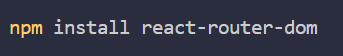
\includegraphics[scale=1]{pics/react-router.PNG}
  \caption{\label{fig:The-caption}React Router installieren }
  \label{fig:impl:use-case-diagramm}
\end{figure}
\\
Als nächstes wird der React Router aufgesetzt. Das ganze findet in dem File App.js statt, was als Basis des Projekts dient.


\begin{lstlisting}[caption=Routen in React]
  function App() {
    return (
      <BrowserRouter>
        <Routes>
          <Route path="/installables" element={<Installables/>}/>
          <Route path="*" element={<PageNotFound/>}/>
        </Routes>
      </BrowserRouter>
    );
}
\end{lstlisting}


Im obigen Code wird \textbf{Routes} und \textbf{Route} von der react-router-dom Library importiert und dann verwendet, um 
die gewünschte Navigation zu implementieren. Alle \textbf{Routen} liegen verschachtelt in den \textbf{Routes}.
Diese haben zwei Hauptparameter:
\begin{itemize}
  \item {\textbf{Path} legt fest, wie der Name schon sagt, auf welchen Pfad der User weitergeleitet werden soll.}
  \item {\textbf{Element} bestimmt, welche Komponente beim Aufruf des Pfades geladen werden soll. Wenn dieser Parameter 
  nicht ausgefüllt ist, wird ein Fehler auftreten.}
\end{itemize}
\newpage
Bis jetzt funktioniert das Routing aber nur durch direkter Änderung der URL. Um die verfügbaren Routen auch mit einem Link 
aufrufen zu können muss \textbf{Link} aus der react-router-dom Library importiert werden. 
Da die Navigationsleiste schon implementiert wurde, kann das Routing per Link gleich in der Navbar-Komponente angelegt werden.

\begin{lstlisting}[caption=Beispiel für Navigation in React]
  const SideBar = () => {
    return (
        <div className="nav-container">
            <Link to="/">
                <img className="doka-logo" src={DokaLogo} alt="Doka" />
            </Link>
            <Link className="nav-link" to="/installablePackages">
                <SideBarIcon />
            </Link>
            <Link className="nav-link" to="/import">
                <SideBarIcon />
            </Link>
        </div>
    );
}
\end{lstlisting}

Das \textbf{to} Attribut legt fest wohin navigiert wird, vorrausgesetzt die Route existiert. siehe Listing 13.
Verschachtelt in den \textbf{Link-Tags} werden Bilder, Icons oder Komponenten eingebettet um ein visuelles Objekt für den User 
zum Klicken anzuzeigen.
\\
\\
Man kann den User natürlich auch programmatisch, nach einem Klick auf einen Button zum Beispiel, auf bestimmte Routen weiterleiten 
mit \textbf{navigate()}.

\begin{lstlisting}[caption=Alternative Navigation]
  <button className="btn" onClick={() => navigate('import')}></button>
\end{lstlisting}
\cite{APCW20020}

\clearpage

\subsection{Authentifizierung}
\setauthor{David Altenhofer}
Beim Aufruf der Seite wird als Erstes geschaut ob der User schon angemeldet beziehungswiese authentifiziert ist.
Dabei wird geschaut ob der LocalStorage, eine gültige Authentifizierung beinhaltet.
Wenn das der Fall ist, dann wird er zur Startseite weitergeleitet. 

Wenn der User aber noch nicht authentifiziert ist, dann kann er sich mit einem 
Login-Button anmelden. Er wird zu einem Login auf \textbf{``https://login.test.doka.com/''} weitergleitet.
Dort kann er sich mit einem gültigen Doka-Konto anmelden.
\\
\begin{figure}[ht!]
  \centering
  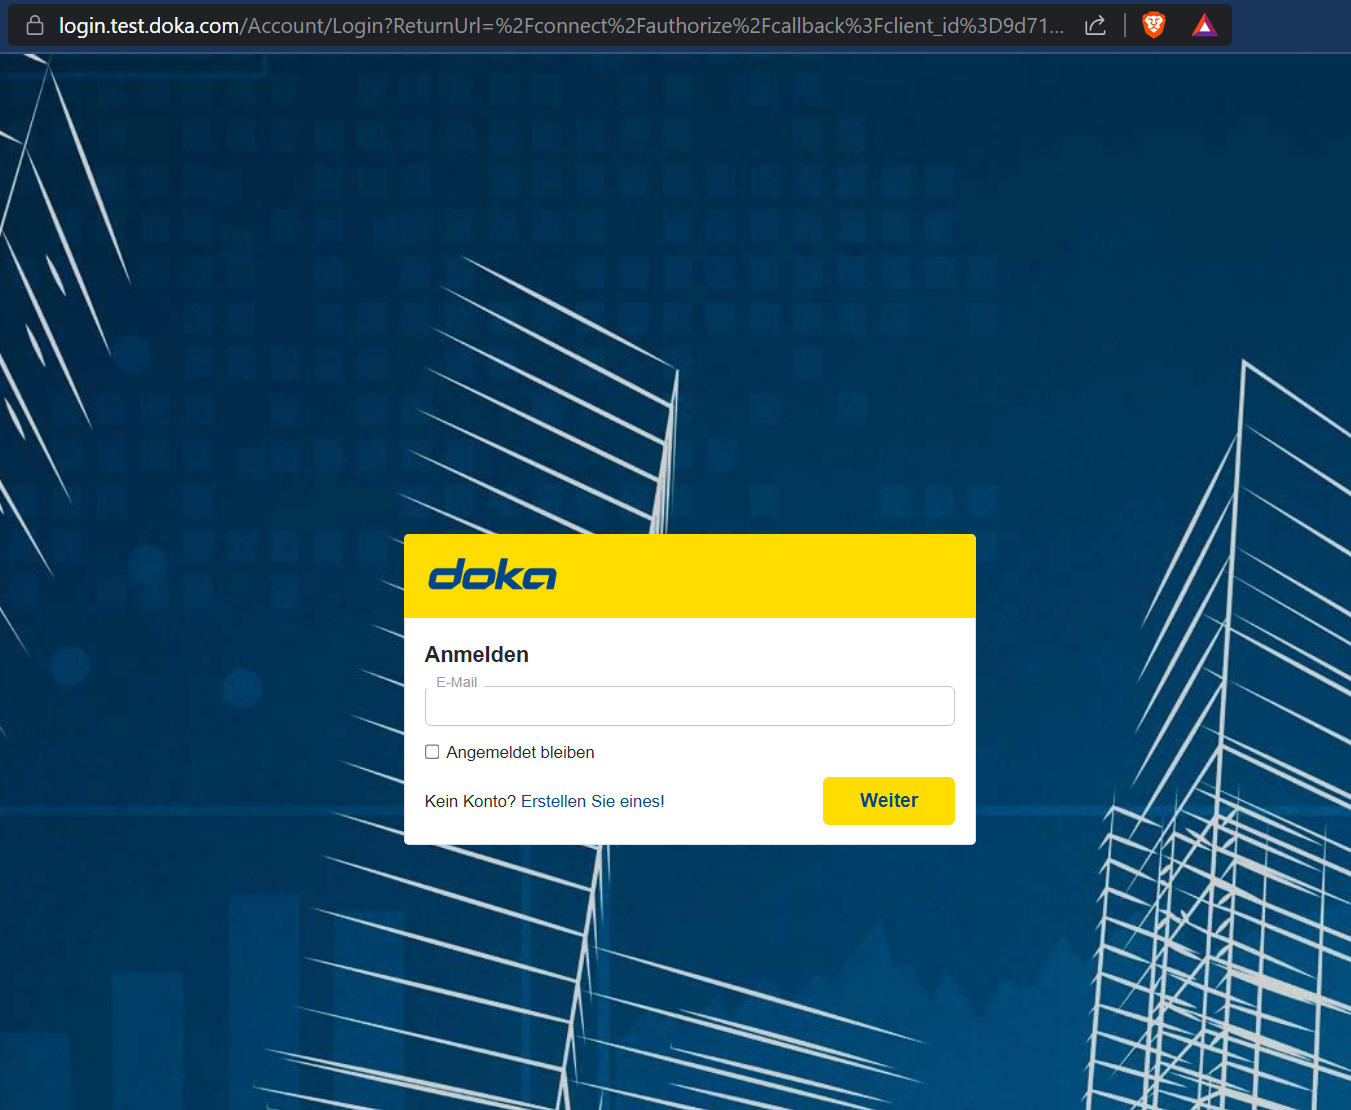
\includegraphics[scale=.5]{pics/doka-login.PNG}
  \caption{\label{fig:The-caption}Doka Login }
  \label{fig:impl:use-case-diagramm}
\end{figure}
\newpage

\subsection*{Das größte Problem dabei}
Das zeitintensivste Problem des ganzen Projektes (zumindest was meinen Teil angeht) war die Authentifizierung hinzubekommen. Grund 
dafür war die völlig neue Technologie von Bearer Tokens und API-Authentifizierung bishin zu den Libraries mit AuthProvidern in React.
Das Grundgerüst für das Ganze war nach eigner Recherche und Besprechung mit den Betreuern relativ schnell implementiert. Anfangs war es 
jedoch so, dass nach der Anmeldung nicht weitergeleitet wurde zu der React-Page, sondern nur eine leere weiße Seite im Browser 
zu sehen war. Die Url hat sich natürlich nicht auf ``http://localhost:3000/'' geändert wie sie sollte, sondern blieb bei der langen Url mit 
den ganzen Parametern wie client-id, scope, sesssion-state usw. 

\subsection*{Die Lösung}
Ich habe lange gebraucht um das Probem zu lösen. Es stellte sich heraus, dass ein simpler Timeout von ungefähr 600 millisekunden 
ausreichen, dass der redirect funktionert. Der Grund dafür ist, dass der Authentifizierungensprozess aufgrund von 
\textbf{asynchroner Verarbeitung} einige Zeit benötigt. Wenn ein direkter Redirect ohne Verzögerung durchgeführt wird, kann es passieren, 
dass der Prozess noch nicht vollständig abgeschlossen ist. Das Hinzufügen eines Timeouts ermöglicht es also den 
Authentifizierungsprozess in dieser Zeitspanne abzuschließen, bevor der Redirect ausgelöst wird.

\begin{lstlisting}[caption=Timeout setzen]
  if (window.location.href.includes('code')) {
            setTimeout(() => {
                window.location.href = window.location.origin;
            }, 600);
        }
\end{lstlisting}
\newpage
\subsection*{Wie funktionert die die Authentifizierung mit Token im Detail?}
\begin{enumerate}
\item Zuerst muss sich beim Identitätsanbieter authentifiziert werden. Das ganze passiert
beim einfachen Anmelden mit einem gültigen Doka-Benutzer. Der Identitätsanbieter stellt dann einen Autorisierungscode aus.\\
\item Nach dem erfolgreichen Anmelden wird der Benutzer zu der angegeben redirect-uri (In dem Fall ``http://localhost:3000'') weitergeleitet.
Die URL enthält einen Autorisierungscode als Parameter. Dieser wird zusammen mit der client-id dafür verwendet, eine Anfrage an den
Identitätsanbieter zu stellen, um einen Zugriffstoken zu erhalten. Dieser Schritt ist jedoch unsichtbar und wird automatisch von der 
Library erledigt. In dem Fall ist das die Library ``react-oidc-context''.\\
\item Nachdem die App den Zugriffstoken erhalten hat, wird speichere ich diesen im Localstorage. Das erlaubt es,
auch nach dem Schließen des Browsers zum Beispiel, immer noch angemeldet zu bleiben.\\
\item Wenn nun eine Anfrage an die geschützte API gesendet wird, fügt man den Bearer Token im
Authorization-Header der Anfrage zurück, und der Zugriff ist gesichert.
\begin{lstlisting}[caption=Authorization-Header]
  let httpOptions = {
    method: 'GET',
    headers: {
        Authorization: localStorage.getItem('access_token')
    }
};
\end{lstlisting}

\end{enumerate}
\newpage

\subsection*{Wie sieht das ganze im Code aus?}
Im index.js File findet die Konfiguration der Authentifizierung statt. Wichtig dabei sind die Login-URL, die client-id, die 
Art des Tokens der zurückgeliefert werden soll und der redirect, also wohin man weitergeleitet wird bei erfolgreicher Anmeldung.
Die App-Komponente mit dem ganzen Inhalt der Website, wird in die AuthProvider-Komponente verschachtelt, in der sich die 
Authentifizierungslogik befindet. 

\begin{lstlisting}[caption=index.js File mit Auth-Parametern]
  import { Auth0Provider } from "react-oidc-context"

const oidcConfig = {
    authority: "https://login.test.doka.com/",
    client_id: "9d71a618-5337-4bff-b8b0-3e236e73e5ea",
    token_type: "Bearer",
    redirect_uri: "http://localhost:3000",
    scope: "openid offline_access profile phone email dfdsin.doka.com/download",
    post_logout_redirect_uri: "http://localhost:3000/login"
}

const root = ReactDOM.createRoot(document.getElementById('root'));
root.render(
    <AuthProvider{...oidcConfig}>
    <App />
    </AuthProvider>
);
\end{lstlisting}

In App.js kann dann der aktuelle Status der Authentifizierungen (isLoading, isAuthenticated,...) abgerufen werden und 
auf Authentifizierungensmethoden wie \textbf{logout} zugegriffen werden. Das ganze funktioniert mit der useAuth-Hook. Das ist 
dann quasi ein Array aus verschieden Variablen, auf das man über mehrere Komponenten Zugriff hat. Sobald die Anmeldung am Doka-Portal 
geglückt ist, wird man zur Startseite der Website weitergeleitet und der Bearer-Token wird im LocalStorage gespeichert. 

\begin{lstlisting}[caption=App.js File - Verwalten des Auth-Status]
  import {useAuth, AuthProvider} from "react-oidc-context"

  function App() {

    const [access_token, setAccess_token] = useState(null);
    const [isAuth, setIsAuth] = useState(false);

    const auth = useAuth();

        if (auth.isLoading) {
            return <div className="box loadingBox"><CircularProgress className="loading"/></div>;
        }

        if (auth.isAuthenticated) {
            const token = 'Bearer ' + auth.user.access_token;
            setAccess_token(token);
            localStorage.setItem('access_token', token);

            return (
                <SideBar />
            )
        } else {
            if (window.location.href !== `${window.location.origin}/login`) {
                return window.location.replace(`${window.location.origin}/login`);
            }
        }
\end{lstlisting}

\section{Retrospektive und Bugfixing}
\setauthor{David Altenhofer}
Da ich bereits 3 Tage vor Ende des Praktikums, mit meinem Teil in React fertig war,
bestand meine Aufgabe darin, den Code nach Fehlfunktionen zu überprüfen und noch einige 
kleine Designänderungen auf Wunsch der Firmenkollegen durchzuführen. Ich habe mich mit 
ihnen über die Zufriedenheit von dem Projekt und unserer Arbeit während des Praktikums 
verständigt und eine Retrospektive über alle Sprints des Projekts durchgeführt. 

In der übrig gebliebenen Zeit, habe ich meinem Diplomarbeitspartner David Precup mit dem neuen Framework geholfen, der 
aufgrund eines längeren Krankenstandes, ziemilch weit hinten war mit seinem Teil im Projekt. 
  
 












	
\begin{spacing}{1}
\chapter{Zusammenfassung}
\end{spacing}
\section{Ergebnis \& Erfahrungen}
Leider können wir das fertige Produkt, aufgrund von internen Firmenkomplikationen nicht 
herzeigen, sondern nur die Herangehensweisen in der Implementation und Durchführung mit den verwendeten
Technologien.

Wir sind mit dem Ergebnis der Diplomarbeit dennoch zufrieden, vorallem wenn man bedenkt, dass 
wir React als komplett neues Framework gelernt haben, um das Projekt 
umzusetzen. Das Praktikum im Sommer bei der Doka GmbH, war aufjedenfall
eine gute Entscheidung und wir haben viel Erfahrung dadurch mitnehmen können. 
Nicht nur das Lernen neuer Technologien, sondern auch das Kennenlernen des Arbeitsklimas in einer so 
großen Firma, haben wir daraus mitgenommen. Obwohl uns natürlich, die Betreuer in der Firma 
als Hilfe zur Verfügung standen, haben wir einen Großteil durch 
eigenhändiges recherchieren im Internet bewältigt. Dadurch haben wir bewiesen, dass wir auch 
ohne Hilfe und außerhalb der Schule, neue technologische Erkenntnisse und Fähigkeiten durch selbstständiges
Arbeiten aneignen können.


\newpage
\pagenumbering{Roman}
\setcounter{page}{\value{RPages}}
\newacronym{guid}{GUID}{Globally Unique Identifier}
\newacronym{jit}{JIT}{Just In Time Compiler}
\newacronym{nfc}{NFC}{Near Field Communication}
\newacronym{rfid}{RFID}{Radio Frequency Identification}

% Usage:
% \gls{label} lowercase in text
% \Gls{label} Uppercase in text
% \newacronym{label}{abbrev}{full}
% \newglossaryentry{label}{settings}



%\setlength{\glsdescwidth}{0.8\linewidth}
\glsnogroupskiptrue
\printglossary[title=Glossar,toctitle=Glossar] %,style=long]
\spacing{1}{
%\bibliographystyle{IEEEtran}
\bibliographystyle{ieeetrande}
\bibliography{bib}
}
\listoffigures
\lstlistoflistings
\appendix
\end{document}

